\documentclass[a4paper]{article}
\addtolength{\hoffset}{-2.25cm}
\addtolength{\textwidth}{4.5cm}
\addtolength{\voffset}{-3.25cm}
\addtolength{\textheight}{5cm}
\setlength{\parindent}{15pt}

\usepackage[unicode=true, colorlinks=false, hidelinks]{hyperref}
\usepackage[utf8]{inputenc}
\usepackage[english, russian]{babel}
\usepackage{mathtext}
\usepackage[T2A, TS1]{fontenc}
\usepackage{microtype} % Slightly tweak font spacing for aesthetics
\usepackage{amsthm, amssymb, amsmath, amsfonts, nccmath}
\usepackage{nicefrac}
\usepackage{epstopdf}
\usepackage[export]{adjustbox}
\usepackage{float} % Improved interface for floating objects
\usepackage{graphicx, multicol} % Enhanced support for graphics
\usepackage{pdfrender,xcolor}
\usepackage{breqn}
\usepackage{mathtools}
\usepackage{titling}
\usepackage{bm}
\usepackage{centernot}
\usepackage[cal=boondoxo,calscaled=.96]{mathalpha}
\usepackage{marvosym, wasysym} % More symbols
\usepackage{rotating} % Rotation tools
\usepackage{censor} % Facilities for controlling restricted text
\usepackage{indentfirst}
\usepackage{svg}

\DeclareMathOperator{\rad}{rad}
\DeclareMathOperator{\imid}{mid}
\DeclareMathOperator{\sign}{sign}
\newcommand{\mbb}[1]{\mathbb{#1}}
\newcommand{\mbf}[1]{\mathbf{#1}}

\usepackage{array}
\newcolumntype{C}[1]{>{\centering\let\newline\\\arraybackslash\hspace{0pt}}m{#1}}

\usepackage{fancyhdr}
\pagestyle{fancy}
\fancyhead{}\renewcommand{\headrulewidth}{0pt}
\fancyfoot[L]{}
\fancyhead{}
\fancyfoot{}
\fancyfoot[R]{\thepage}
\begin{document}
\large
\begin{center}
    Санкт-Петербургский политехнический университет\\
    Высшая школа прикладной математики и\\вычислительной физики,\\ 
    Физико-механический институт\\
    \vspace{3em}
    Направление подготовки\\
    01.03.02 «Прикладная математика и информатика»\\
    \vspace{10em}
    \Large
    Отчет по лабораторной работе №5 \\
    по дисциплине «Интервальный анализ»
    \vspace{19em}
    \large
\end{center}
Выполнил студент гр. 5030102/80201\\
Кирпиченко С. Р.\\
Руководитель\\
Баженов А. Н.
\vspace{10em}
\begin{center}
    Санкт-Петербург\\
    2021
\end{center}
\thispagestyle{empty}
\newpage
\tableofcontents
\addtocontents{toc}{~\hfill\textbf{Страница}\par}
\newpage
\listoffigures
\addtocontents{lof}{~\hfill\textbf{Страница}\par}
\newpage
\section{Постановка задачи}
Для линейной задачи построения регрессии $\mathbf{y}=X\beta$ необходимо задать набор значений $x$ и $\mbf{y}$ с некоторыми ошибками измерений по отклику. Необходимо провести вычисления и привести иллюстрации:
\begin{itemize}
    \item Построить интервальное множество решений $\beta$, сделать точечные оценки параметров.
    \item Построить коридор совместных зависимостей.
    \item Задать набор предсказания внутри и вне $x$, построить набор значений выходной переменной $\mbf{y}$.
\end{itemize}
\section{Теория}
\subsection{Решение задачи регрессии с интервальным откликом}
Решением задачи восстановления зависимости можно считать любое (в данном случае линейное) решение, проходящее через все исходные брусы.
\subsection{Информационное множество}
Интервальное множество решений $\beta$, которое необходимо построить и оценить в задании 1, называется информационным множеством.
В качестве точечных оценок информационного множества будут использованы следующие величины:
\begin{itemize}
    \item Середина наибольшей диагонали
    \item Центр тяжести (среднее суммы всех вершин)
    \item Оценка $\beta$, полученная решением исходной задачи в точечной постановке (с серединами интервалов) методом наименьших квадратов
\end{itemize}
\subsection{Коридор совместных зависимостей}
Коридором совместных зависимостей называется множество, образованное всеми решениями с параметрами из информационного множества.
\subsection{Предсказание значений}
Предсказание осуществляется посредством построения сечения коридора совместных зависимостей в указанных точках.
Соотношение прогнозных и исходных интервалов в исходных точках измерений является одним из показателей качества построенной модели.
\section{Реализация}
Для осуществления вычислений и визуализации результатов использовалась среда Octave с библиотекой С. И. Жилина.
\section{Результаты}
В качестве входных значений предиктора были выбраны точки $x=\{2,4,10,12\}$. В качестве отклика $\mbf{y}$ были взяты значения $[y_i-\varepsilon_i,\:y_i+\varepsilon_i]$, где $y=\{2,8.5,18,25\}$, $\varepsilon=\{2,1.5,2.5,1.5\}$. $\hat{\beta}_{\mathrm{max diag}}=(-0.95, 2.1)$, $\hat{\beta}_{\mathrm{gravity}}=(-0.8188, 2.08)$, $\hat{\beta}_{\mathrm{lsm}}=(-1.39, 2.11)$.
\begin{figure}[H]
    \centering
    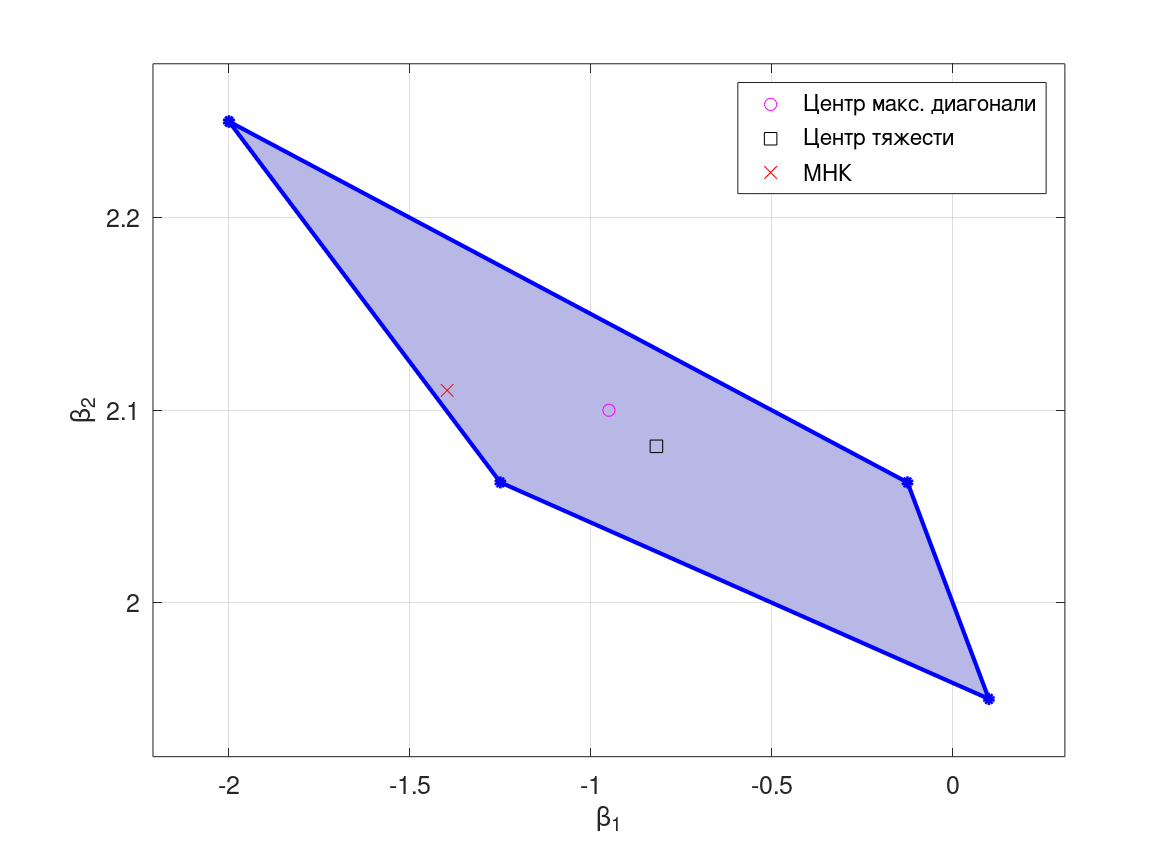
\includegraphics[width=14cm]{img/info.png}
    \caption{Информационное множество с точечными оценками}
    \label{fig:info}
\end{figure}
Коридор совместных зависимостей обозначен фиолетовым цветом на следующем графике.
\begin{figure}[H]
    \centering
    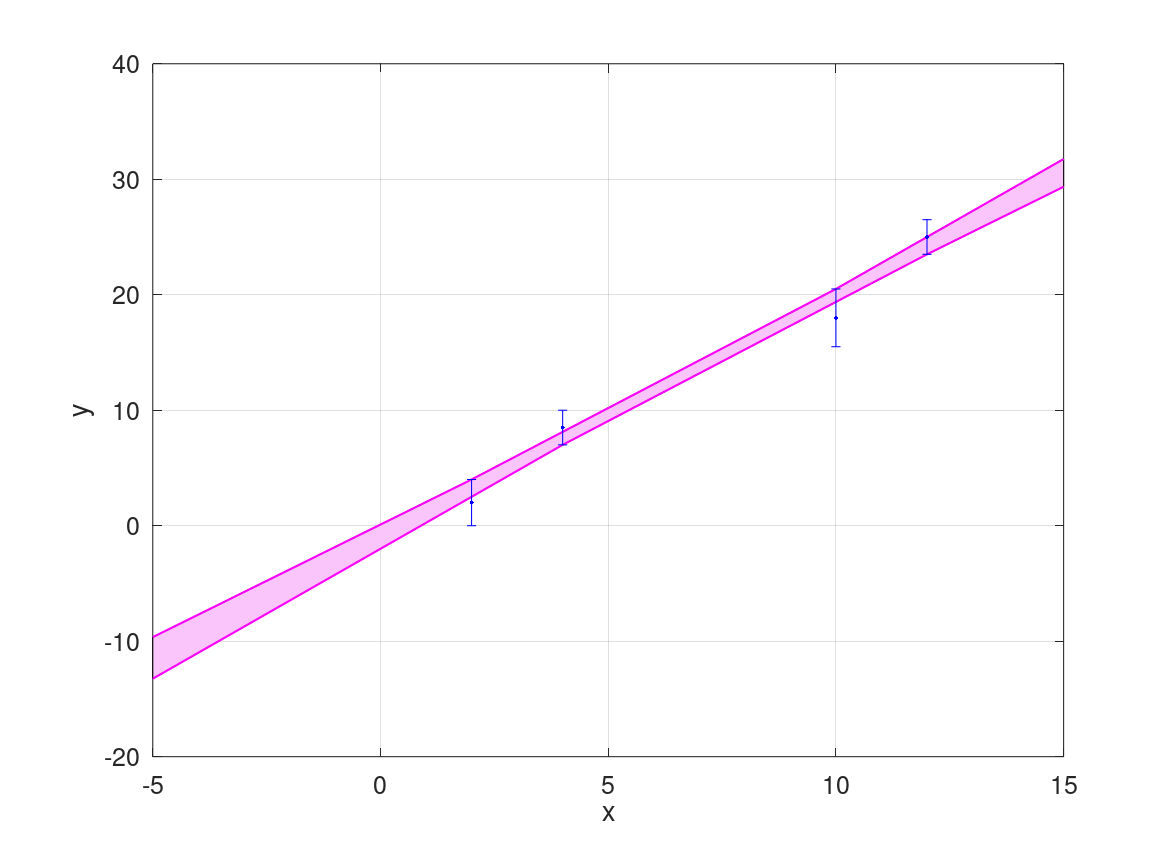
\includegraphics[width=13cm]{img/reg.png}
    \caption{Коридор совместных зависимостей и исходные измерения}
    \label{fig:reg}
\end{figure}
Для построения следующего графика были выбраны точки $x_p=\{2,10,-1,5,13\}$ для вычисления предсказаний. Первые две из них принадлежат множеству точек, по которым строилась регрессия. Синими отрезками обозначены образующие модель интервалы, черными - предсказания.
\begin{figure}[H]
    \centering
    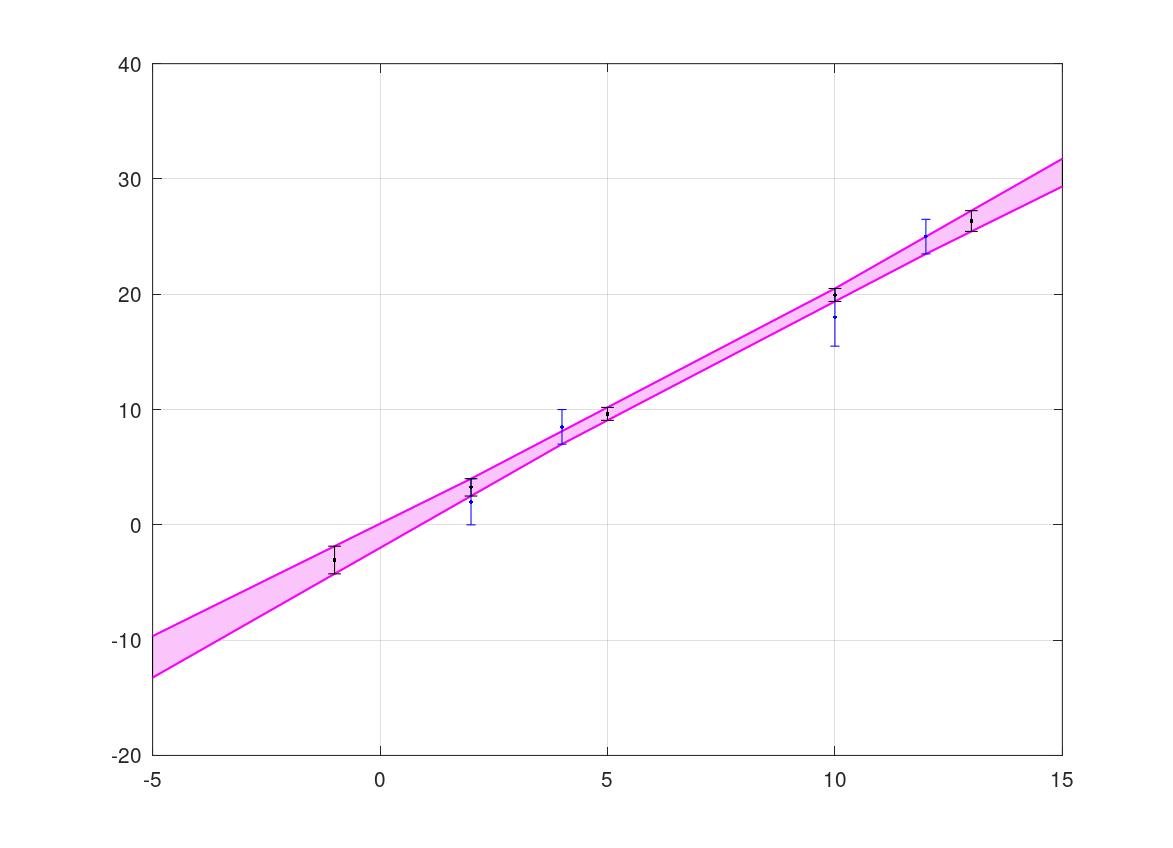
\includegraphics[width=15cm]{img/pred.png}
    \caption{График построенной модели регрессии с предсказаниями}
    \label{fig:pred}
\end{figure}
\section{Обсуждение}
\begin{enumerate}
    \item По форме информационного множества можно сделать вывод, что все 4 интервала оказывают влияние на построенную модель.
    \item Точечные оценки информационного множества дали ощутимо разные результаты. Все три оценки лежат внутри множества, однако оценка, полученная на основании МНК, находится возле границы. В общем случае возможно подобрать данные так, чтобы данная оценка вышла за пределы информационного множества.
    \item По графику \ref{fig:reg} видно, что исходные данные имеют значительную неопределенность и разброс, коридор совместных зависимостей испытывает влияние всех интервалов и довольно узок в средней части.
    \item По предсказаниям, полученным в точках, являющихся подмножеством $x$, видно, что исходные и предсказанные интервалы довольно сильно различаются. Можно сделать вывод, что линейная модель не очень хорошо описывает исходные данные. Тем не менее, в целом предсказания получились с невысокой степенью неопределенности.
\end{enumerate}
\section*{Исходный код}
С исходным кодом программы и отчета можно ознакомиться в репозитории \url{https://github.com/Stasychbr/IntervalArith}.
\end{document}
